\documentclass[conference,letterpaper]{IEEEtran}
\IEEEoverridecommandlockouts
\usepackage{cite}
\usepackage{amsmath,amssymb,amsfonts,amsthm}
\usepackage{graphicx}
\usepackage{booktabs}
\usepackage{array}
\usepackage{xcolor}
\usepackage{url}
\usepackage[hidelinks]{hyperref}

\newtheorem{theorem}{Theorem}
\newtheorem{corollary}{Corollary}
\newtheorem{proposition}{Proposition}
\newtheorem{lemma}{Lemma}
\theoremstyle{definition}
\newtheorem{definition}{Definition}
\newtheorem{example}{Example}
\newtheorem{conjecture}{Conjecture}

\newcommand{\Prb}{\mathbb{P}}
\newcommand{\E}{\mathbb{E}}
\newcommand{\RQ}[1]{\textbf{RQ#1}}
\newcommand{\pp}{\,pp}
\newcommand{\IIDp}{\textup{\textsc{IID}}}
\newcommand{\PAIRp}{\textup{\textsc{Pair}}}
\newcommand{\GATEp}{\textup{\textsc{Gate}}}
\newcommand{\STRICTp}{\textup{\textsc{Strict}}}
\newcommand{\NTargets}{289}
\newcommand{\NVictims}{231}
\newcommand{\NBrittles}{58}
\newcommand{\NExact}{258}
\newcommand{\NMC}{31}
\newcommand{\NBzero}{211}
\newcommand{\NZeroGap}{0}
\newcommand{\NMCneg}{31}
\newcommand{\NMCpos}{0}
\newcommand{\NMCund}{0}
\newcommand{\NConsistent}{181}
\newcommand{\NInconsistent}{108}
\newcommand{\NflowTen}{71}
\newcommand{\FMean}{41.7}
\newcommand{\FMedian}{50.0}
\newcommand{\FMin}{1.2}
\newcommand{\KRSaveMean}{0.40}
\newcommand{\KRSaveMax}{0.50}
\newcommand{\KRSaveMedian}{0.50}
\newcommand{\KRSaveCIlo}{0.395}
\newcommand{\KRSaveCIhi}{0.395}
\newcommand{\KRSaveAtLimit}{211}
\newcommand{\KRSaveRelMean}{12.5}
\newcommand{\KRSaveRelMedian}{11.1}
\newcommand{\KRRunsIID}{10.22}
\newcommand{\KRRunsPair}{9.82}
\newcommand{\KRGainTwo}{11.18}
\newcommand{\KRMaxGainTwo}{25.00}
\newcommand{\KRShareLowTwo}{55}
\newcommand{\KRIidTwo}{58.0}
\newcommand{\KRPairTwo}{69.1}
\newcommand{\KRGateTwo}{60.3}
\newcommand{\KRStrictTwo}{60.3}
\newcommand{\KRPairMinusIidTwo}{+11.19}
\newcommand{\KRPairMinusIidCITwo}{0.04}
\newcommand{\KRGateMinusIidTwo}{+2.31}
\newcommand{\KRGateMinusIidCITwo}{0.02}
\newcommand{\KRPairMinusGateTwo}{+8.88}
\newcommand{\KRPairMinusGateCITwo}{0.03}
\newcommand{\KRStrictMinusIidTwo}{+2.31}
\newcommand{\KRStrictMinusIidCITwo}{0.02}
\newcommand{\KRGateWorseTwo}{0}
\newcommand{\KRGateBetterTwo}{39}
\newcommand{\KRPairWorseGateTwo}{4}
\newcommand{\KRPairBetterGateTwo}{23}
\newcommand{\KRPairWorseIidTwo}{0}
\newcommand{\KRConsPairMinusIidTwo}{+9.08}
\newcommand{\KRConsGateMinusIidTwo}{+2.78}
\newcommand{\KRMWPairMinusIidTwo}{+9.43}
\newcommand{\KRMWGateMinusIidTwo}{+5.52}
\newcommand{\KRGainFour}{3.51}
\newcommand{\KRMaxGainFour}{8.64}
\newcommand{\KRShareLowFour}{74}
\newcommand{\KRIidFour}{71.2}
\newcommand{\KRPairFour}{74.8}
\newcommand{\KRGateFour}{74.4}
\newcommand{\KRStrictFour}{72.5}
\newcommand{\KRPairMinusIidFour}{+3.54}
\newcommand{\KRPairMinusIidCIFour}{0.02}
\newcommand{\KRGateMinusIidFour}{+3.14}
\newcommand{\KRGateMinusIidCIFour}{0.02}
\newcommand{\KRPairMinusGateFour}{+0.40}
\newcommand{\KRPairMinusGateCIFour}{0.01}
\newcommand{\KRStrictMinusIidFour}{+1.25}
\newcommand{\KRStrictMinusIidCIFour}{0.01}
\newcommand{\KRGateWorseFour}{0}
\newcommand{\KRGateBetterFour}{44}
\newcommand{\KRPairWorseGateFour}{5}
\newcommand{\KRPairBetterGateFour}{8}
\newcommand{\KRPairWorseIidFour}{0}
\newcommand{\KRConsPairMinusIidFour}{+3.26}
\newcommand{\KRConsGateMinusIidFour}{+2.77}
\newcommand{\KRMWPairMinusIidFour}{+3.13}
\newcommand{\KRMWGateMinusIidFour}{+2.98}
\newcommand{\KRGainTen}{0.46}
\newcommand{\KRMaxGainTen}{2.99}
\newcommand{\KRShareLowTen}{94}
\newcommand{\KRIidTen}{81.2}
\newcommand{\KRPairTen}{81.7}
\newcommand{\KRGateTen}{81.7}
\newcommand{\KRStrictTen}{81.5}
\newcommand{\KRPairMinusIidTen}{+0.46}
\newcommand{\KRPairMinusIidCITen}{0.01}
\newcommand{\KRGateMinusIidTen}{+0.43}
\newcommand{\KRGateMinusIidCITen}{0.01}
\newcommand{\KRPairMinusGateTen}{+0.02}
\newcommand{\KRPairMinusGateCITen}{0.00}
\newcommand{\KRStrictMinusIidTen}{+0.30}
\newcommand{\KRStrictMinusIidCITen}{0.01}
\newcommand{\KRGateWorseTen}{0}
\newcommand{\KRGateBetterTen}{37}
\newcommand{\KRPairWorseGateTen}{5}
\newcommand{\KRPairBetterGateTen}{8}
\newcommand{\KRPairWorseIidTen}{0}
\newcommand{\KRConsPairMinusIidTen}{+0.62}
\newcommand{\KRConsGateMinusIidTen}{+0.59}
\newcommand{\KRMWPairMinusIidTen}{+0.73}
\newcommand{\KRMWGateMinusIidTen}{+0.72}
\newcommand{\KRGainTwenty}{0.19}
\newcommand{\KRMaxGainTwenty}{1.42}
\newcommand{\KRShareLowTwenty}{98}
\newcommand{\KRIidTwenty}{86.9}
\newcommand{\KRPairTwenty}{87.1}
\newcommand{\KRGateTwenty}{87.1}
\newcommand{\KRStrictTwenty}{87.1}
\newcommand{\KRPairMinusIidTwenty}{+0.19}
\newcommand{\KRPairMinusIidCITwenty}{0.01}
\newcommand{\KRGateMinusIidTwenty}{+0.18}
\newcommand{\KRGateMinusIidCITwenty}{0.01}
\newcommand{\KRPairMinusGateTwenty}{+0.00}
\newcommand{\KRPairMinusGateCITwenty}{0.00}
\newcommand{\KRStrictMinusIidTwenty}{+0.16}
\newcommand{\KRStrictMinusIidCITwenty}{0.01}
\newcommand{\KRGateWorseTwenty}{0}
\newcommand{\KRGateBetterTwenty}{23}
\newcommand{\KRPairWorseGateTwenty}{5}
\newcommand{\KRPairBetterGateTwenty}{3}
\newcommand{\KRPairWorseIidTwenty}{0}
\newcommand{\KRConsPairMinusIidTwenty}{+0.29}
\newcommand{\KRConsGateMinusIidTwenty}{+0.28}
\newcommand{\KRMWPairMinusIidTwenty}{+0.32}
\newcommand{\KRMWGateMinusIidTwenty}{+0.32}
\newcommand{\KRGainForty}{0.13}
\newcommand{\KRMaxGainForty}{0.69}
\newcommand{\KRShareLowForty}{100}
\newcommand{\KRIidForty}{92.8}
\newcommand{\KRPairForty}{92.9}
\newcommand{\KRGateForty}{92.9}
\newcommand{\KRStrictForty}{92.8}
\newcommand{\KRPairMinusIidForty}{+0.13}
\newcommand{\KRPairMinusIidCIForty}{0.01}
\newcommand{\KRGateMinusIidForty}{+0.12}
\newcommand{\KRGateMinusIidCIForty}{0.01}
\newcommand{\KRPairMinusGateForty}{+0.00}
\newcommand{\KRPairMinusGateCIForty}{0.00}
\newcommand{\KRStrictMinusIidForty}{+0.09}
\newcommand{\KRStrictMinusIidCIForty}{0.01}
\newcommand{\KRGateWorseForty}{0}
\newcommand{\KRGateBetterForty}{15}
\newcommand{\KRPairWorseGateForty}{3}
\newcommand{\KRPairBetterGateForty}{1}
\newcommand{\KRPairWorseIidForty}{0}
\newcommand{\KRConsPairMinusIidForty}{+0.19}
\newcommand{\KRConsGateMinusIidForty}{+0.19}
\newcommand{\KRMWPairMinusIidForty}{+0.14}
\newcommand{\KRMWGateMinusIidForty}{+0.14}
\newcommand{\NRSaveMean}{0.70}
\newcommand{\NRSaveMax}{1.00}
\newcommand{\NRSaveMedian}{0.67}
\newcommand{\NRSaveCIlo}{0.702}
\newcommand{\NRSaveCIhi}{0.702}
\newcommand{\NRSaveAtLimit}{94}
\newcommand{\NRSaveRelMean}{16.9}
\newcommand{\NRSaveRelMedian}{19.0}
\newcommand{\NRRunsIID}{12.62}
\newcommand{\NRRunsPair}{11.91}
\newcommand{\NRGainTwo}{22.37}
\newcommand{\NRMaxGainTwo}{50.00}
\newcommand{\NRShareLowTwo}{34}
\newcommand{\NRIidTwo}{32.5}
\newcommand{\NRPairTwo}{54.9}
\newcommand{\NRGateTwo}{54.9}
\newcommand{\NRStrictTwo}{34.8}
\newcommand{\NRPairMinusIidTwo}{+22.40}
\newcommand{\NRPairMinusIidCITwo}{0.04}
\newcommand{\NRGateMinusIidTwo}{+22.40}
\newcommand{\NRGateMinusIidCITwo}{0.04}
\newcommand{\NRPairMinusGateTwo}{+0.00}
\newcommand{\NRPairMinusGateCITwo}{0.00}
\newcommand{\NRStrictMinusIidTwo}{+2.31}
\newcommand{\NRStrictMinusIidCITwo}{0.02}
\newcommand{\NRGateWorseTwo}{0}
\newcommand{\NRGateBetterTwo}{45}
\newcommand{\NRPairWorseGateTwo}{0}
\newcommand{\NRPairBetterGateTwo}{0}
\newcommand{\NRPairWorseIidTwo}{0}
\newcommand{\NRConsPairMinusIidTwo}{+18.23}
\newcommand{\NRConsGateMinusIidTwo}{+18.23}
\newcommand{\NRMWPairMinusIidTwo}{+18.89}
\newcommand{\NRMWGateMinusIidTwo}{+18.89}
\newcommand{\NRGainFour}{6.91}
\newcommand{\NRMaxGainFour}{12.50}
\newcommand{\NRShareLowFour}{51}
\newcommand{\NRIidFour}{57.9}
\newcommand{\NRPairFour}{64.9}
\newcommand{\NRGateFour}{64.4}
\newcommand{\NRStrictFour}{59.2}
\newcommand{\NRPairMinusIidFour}{+6.94}
\newcommand{\NRPairMinusIidCIFour}{0.03}
\newcommand{\NRGateMinusIidFour}{+6.48}
\newcommand{\NRGateMinusIidCIFour}{0.03}
\newcommand{\NRPairMinusGateFour}{+0.46}
\newcommand{\NRPairMinusGateCIFour}{0.01}
\newcommand{\NRStrictMinusIidFour}{+1.25}
\newcommand{\NRStrictMinusIidCIFour}{0.01}
\newcommand{\NRGateWorseFour}{0}
\newcommand{\NRGateBetterFour}{45}
\newcommand{\NRPairWorseGateFour}{5}
\newcommand{\NRPairBetterGateFour}{15}
\newcommand{\NRPairWorseIidFour}{0}
\newcommand{\NRConsPairMinusIidFour}{+6.12}
\newcommand{\NRConsGateMinusIidFour}{+5.57}
\newcommand{\NRMWPairMinusIidFour}{+6.42}
\newcommand{\NRMWGateMinusIidFour}{+6.20}
\newcommand{\NRGainTen}{0.85}
\newcommand{\NRMaxGainTen}{2.99}
\newcommand{\NRShareLowTen}{72}
\newcommand{\NRIidTen}{75.5}
\newcommand{\NRPairTen}{76.4}
\newcommand{\NRGateTen}{76.4}
\newcommand{\NRStrictTen}{75.8}
\newcommand{\NRPairMinusIidTen}{+0.85}
\newcommand{\NRPairMinusIidCITen}{0.02}
\newcommand{\NRGateMinusIidTen}{+0.86}
\newcommand{\NRGateMinusIidCITen}{0.02}
\newcommand{\NRPairMinusGateTen}{-0.01}
\newcommand{\NRPairMinusGateCITen}{0.00}
\newcommand{\NRStrictMinusIidTen}{+0.30}
\newcommand{\NRStrictMinusIidCITen}{0.01}
\newcommand{\NRGateWorseTen}{0}
\newcommand{\NRGateBetterTen}{45}
\newcommand{\NRPairWorseGateTen}{5}
\newcommand{\NRPairBetterGateTen}{14}
\newcommand{\NRPairWorseIidTen}{0}
\newcommand{\NRConsPairMinusIidTen}{+0.86}
\newcommand{\NRConsGateMinusIidTen}{+0.78}
\newcommand{\NRMWPairMinusIidTen}{+1.21}
\newcommand{\NRMWGateMinusIidTen}{+1.21}
\newcommand{\NRGainTwenty}{0.33}
\newcommand{\NRMaxGainTwenty}{1.42}
\newcommand{\NRShareLowTwenty}{81}
\newcommand{\NRIidTwenty}{84.0}
\newcommand{\NRPairTwenty}{84.4}
\newcommand{\NRGateTwenty}{84.5}
\newcommand{\NRStrictTwenty}{84.2}
\newcommand{\NRPairMinusIidTwenty}{+0.33}
\newcommand{\NRPairMinusIidCITwenty}{0.02}
\newcommand{\NRGateMinusIidTwenty}{+0.43}
\newcommand{\NRGateMinusIidCITwenty}{0.02}
\newcommand{\NRPairMinusGateTwenty}{-0.10}
\newcommand{\NRPairMinusGateCITwenty}{0.00}
\newcommand{\NRStrictMinusIidTwenty}{+0.16}
\newcommand{\NRStrictMinusIidCITwenty}{0.01}
\newcommand{\NRGateWorseTwenty}{0}
\newcommand{\NRGateBetterTwenty}{36}
\newcommand{\NRPairWorseGateTwenty}{6}
\newcommand{\NRPairBetterGateTwenty}{9}
\newcommand{\NRPairWorseIidTwenty}{0}
\newcommand{\NRConsPairMinusIidTwenty}{+0.31}
\newcommand{\NRConsGateMinusIidTwenty}{+0.27}
\newcommand{\NRMWPairMinusIidTwenty}{+0.43}
\newcommand{\NRMWGateMinusIidTwenty}{+0.49}
\newcommand{\NRGainForty}{0.18}
\newcommand{\NRMaxGainForty}{0.69}
\newcommand{\NRShareLowForty}{87}
\newcommand{\NRIidForty}{91.7}
\newcommand{\NRPairForty}{91.9}
\newcommand{\NRGateForty}{92.0}
\newcommand{\NRStrictForty}{91.8}
\newcommand{\NRPairMinusIidForty}{+0.18}
\newcommand{\NRPairMinusIidCIForty}{0.01}
\newcommand{\NRGateMinusIidForty}{+0.24}
\newcommand{\NRGateMinusIidCIForty}{0.01}
\newcommand{\NRPairMinusGateForty}{-0.06}
\newcommand{\NRPairMinusGateCIForty}{0.01}
\newcommand{\NRStrictMinusIidForty}{+0.09}
\newcommand{\NRStrictMinusIidCIForty}{0.01}
\newcommand{\NRGateWorseForty}{0}
\newcommand{\NRGateBetterForty}{19}
\newcommand{\NRPairWorseGateForty}{6}
\newcommand{\NRPairBetterGateForty}{2}
\newcommand{\NRPairWorseIidForty}{0}
\newcommand{\NRConsPairMinusIidForty}{+0.20}
\newcommand{\NRConsGateMinusIidForty}{+0.17}
\newcommand{\NRMWPairMinusIidForty}{+0.16}
\newcommand{\NRMWGateMinusIidForty}{+0.20}
\newcommand{\Runs}{100{,}000}

\newcommand{\NTargetsAlt}{289}
\newcommand{\NVictimsAlt}{231}
\newcommand{\NBrittlesAlt}{58}
\newcommand{\NExactAlt}{254}
\newcommand{\NMCAlt}{35}
\newcommand{\NBzeroAlt}{211}
\newcommand{\NZeroGapAlt}{0}
\newcommand{\NMCnegAlt}{35}
\newcommand{\NMCposAlt}{0}
\newcommand{\NMCundAlt}{0}
\newcommand{\NConsistentAlt}{181}
\newcommand{\NInconsistentAlt}{108}
\newcommand{\NflowTenAlt}{71}
\newcommand{\FMeanAlt}{41.7}
\newcommand{\FMedianAlt}{50.0}
\newcommand{\FMinAlt}{1.2}
\newcommand{\KRSaveMeanAlt}{0.40}
\newcommand{\KRSaveMaxAlt}{0.50}
\newcommand{\KRSaveMedianAlt}{0.50}
\newcommand{\KRSaveCIloAlt}{0.395}
\newcommand{\KRSaveCIhiAlt}{0.395}
\newcommand{\KRSaveAtLimitAlt}{211}
\newcommand{\KRSaveRelMeanAlt}{12.5}
\newcommand{\KRSaveRelMedianAlt}{11.1}
\newcommand{\KRRunsIIDAlt}{10.22}
\newcommand{\KRRunsPairAlt}{9.82}
\newcommand{\KRGainTwoAlt}{11.18}
\newcommand{\KRMaxGainTwoAlt}{25.00}
\newcommand{\KRShareLowTwoAlt}{55}
\newcommand{\KRIidTwoAlt}{58.0}
\newcommand{\KRPairTwoAlt}{69.1}
\newcommand{\KRGateTwoAlt}{60.3}
\newcommand{\KRStrictTwoAlt}{60.3}
\newcommand{\KRPairMinusIidTwoAlt}{+11.17}
\newcommand{\KRPairMinusIidCITwoAlt}{0.05}
\newcommand{\KRGateMinusIidTwoAlt}{+2.29}
\newcommand{\KRGateMinusIidCITwoAlt}{0.03}
\newcommand{\KRPairMinusGateTwoAlt}{+8.88}
\newcommand{\KRPairMinusGateCITwoAlt}{0.05}
\newcommand{\KRStrictMinusIidTwoAlt}{+2.29}
\newcommand{\KRStrictMinusIidCITwoAlt}{0.03}
\newcommand{\KRGateWorseTwoAlt}{0}
\newcommand{\KRGateBetterTwoAlt}{36}
\newcommand{\KRPairWorseGateTwoAlt}{4}
\newcommand{\KRPairBetterGateTwoAlt}{22}
\newcommand{\KRPairWorseIidTwoAlt}{0}
\newcommand{\KRConsPairMinusIidTwoAlt}{+9.11}
\newcommand{\KRConsGateMinusIidTwoAlt}{+2.75}
\newcommand{\KRMWPairMinusIidTwoAlt}{+9.44}
\newcommand{\KRMWGateMinusIidTwoAlt}{+5.52}
\newcommand{\KRGainFourAlt}{3.51}
\newcommand{\KRMaxGainFourAlt}{8.64}
\newcommand{\KRShareLowFourAlt}{74}
\newcommand{\KRIidFourAlt}{71.3}
\newcommand{\KRPairFourAlt}{74.8}
\newcommand{\KRGateFourAlt}{74.4}
\newcommand{\KRStrictFourAlt}{72.5}
\newcommand{\KRPairMinusIidFourAlt}{+3.50}
\newcommand{\KRPairMinusIidCIFourAlt}{0.03}
\newcommand{\KRGateMinusIidFourAlt}{+3.10}
\newcommand{\KRGateMinusIidCIFourAlt}{0.03}
\newcommand{\KRPairMinusGateFourAlt}{+0.40}
\newcommand{\KRPairMinusGateCIFourAlt}{0.01}
\newcommand{\KRStrictMinusIidFourAlt}{+1.25}
\newcommand{\KRStrictMinusIidCIFourAlt}{0.02}
\newcommand{\KRGateWorseFourAlt}{0}
\newcommand{\KRGateBetterFourAlt}{40}
\newcommand{\KRPairWorseGateFourAlt}{5}
\newcommand{\KRPairBetterGateFourAlt}{7}
\newcommand{\KRPairWorseIidFourAlt}{0}
\newcommand{\KRConsPairMinusIidFourAlt}{+3.25}
\newcommand{\KRConsGateMinusIidFourAlt}{+2.75}
\newcommand{\KRMWPairMinusIidFourAlt}{+3.10}
\newcommand{\KRMWGateMinusIidFourAlt}{+2.96}
\newcommand{\KRGainTenAlt}{0.46}
\newcommand{\KRMaxGainTenAlt}{2.99}
\newcommand{\KRShareLowTenAlt}{94}
\newcommand{\KRIidTenAlt}{81.2}
\newcommand{\KRPairTenAlt}{81.7}
\newcommand{\KRGateTenAlt}{81.7}
\newcommand{\KRStrictTenAlt}{81.5}
\newcommand{\KRPairMinusIidTenAlt}{+0.46}
\newcommand{\KRPairMinusIidCITenAlt}{0.02}
\newcommand{\KRGateMinusIidTenAlt}{+0.44}
\newcommand{\KRGateMinusIidCITenAlt}{0.02}
\newcommand{\KRPairMinusGateTenAlt}{+0.03}
\newcommand{\KRPairMinusGateCITenAlt}{0.00}
\newcommand{\KRStrictMinusIidTenAlt}{+0.30}
\newcommand{\KRStrictMinusIidCITenAlt}{0.02}
\newcommand{\KRGateWorseTenAlt}{0}
\newcommand{\KRGateBetterTenAlt}{34}
\newcommand{\KRPairWorseGateTenAlt}{5}
\newcommand{\KRPairBetterGateTenAlt}{6}
\newcommand{\KRPairWorseIidTenAlt}{0}
\newcommand{\KRConsPairMinusIidTenAlt}{+0.64}
\newcommand{\KRConsGateMinusIidTenAlt}{+0.60}
\newcommand{\KRMWPairMinusIidTenAlt}{+0.74}
\newcommand{\KRMWGateMinusIidTenAlt}{+0.73}
\newcommand{\KRGainTwentyAlt}{0.19}
\newcommand{\KRMaxGainTwentyAlt}{1.42}
\newcommand{\KRShareLowTwentyAlt}{98}
\newcommand{\KRIidTwentyAlt}{86.9}
\newcommand{\KRPairTwentyAlt}{87.1}
\newcommand{\KRGateTwentyAlt}{87.1}
\newcommand{\KRStrictTwentyAlt}{87.1}
\newcommand{\KRPairMinusIidTwentyAlt}{+0.19}
\newcommand{\KRPairMinusIidCITwentyAlt}{0.02}
\newcommand{\KRGateMinusIidTwentyAlt}{+0.19}
\newcommand{\KRGateMinusIidCITwentyAlt}{0.02}
\newcommand{\KRPairMinusGateTwentyAlt}{+0.00}
\newcommand{\KRPairMinusGateCITwentyAlt}{0.00}
\newcommand{\KRStrictMinusIidTwentyAlt}{+0.16}
\newcommand{\KRStrictMinusIidCITwentyAlt}{0.02}
\newcommand{\KRGateWorseTwentyAlt}{0}
\newcommand{\KRGateBetterTwentyAlt}{23}
\newcommand{\KRPairWorseGateTwentyAlt}{5}
\newcommand{\KRPairBetterGateTwentyAlt}{2}
\newcommand{\KRPairWorseIidTwentyAlt}{0}
\newcommand{\KRConsPairMinusIidTwentyAlt}{+0.30}
\newcommand{\KRConsGateMinusIidTwentyAlt}{+0.30}
\newcommand{\KRMWPairMinusIidTwentyAlt}{+0.31}
\newcommand{\KRMWGateMinusIidTwentyAlt}{+0.31}
\newcommand{\KRGainFortyAlt}{0.13}
\newcommand{\KRMaxGainFortyAlt}{0.69}
\newcommand{\KRShareLowFortyAlt}{100}
\newcommand{\KRIidFortyAlt}{92.8}
\newcommand{\KRPairFortyAlt}{92.9}
\newcommand{\KRGateFortyAlt}{92.9}
\newcommand{\KRStrictFortyAlt}{92.9}
\newcommand{\KRPairMinusIidFortyAlt}{+0.13}
\newcommand{\KRPairMinusIidCIFortyAlt}{0.02}
\newcommand{\KRGateMinusIidFortyAlt}{+0.13}
\newcommand{\KRGateMinusIidCIFortyAlt}{0.02}
\newcommand{\KRPairMinusGateFortyAlt}{+0.00}
\newcommand{\KRPairMinusGateCIFortyAlt}{0.00}
\newcommand{\KRStrictMinusIidFortyAlt}{+0.09}
\newcommand{\KRStrictMinusIidCIFortyAlt}{0.02}
\newcommand{\KRGateWorseFortyAlt}{0}
\newcommand{\KRGateBetterFortyAlt}{15}
\newcommand{\KRPairWorseGateFortyAlt}{3}
\newcommand{\KRPairBetterGateFortyAlt}{1}
\newcommand{\KRPairWorseIidFortyAlt}{0}
\newcommand{\KRConsPairMinusIidFortyAlt}{+0.20}
\newcommand{\KRConsGateMinusIidFortyAlt}{+0.20}
\newcommand{\KRMWPairMinusIidFortyAlt}{+0.15}
\newcommand{\KRMWGateMinusIidFortyAlt}{+0.15}
\newcommand{\NRSaveMeanAlt}{0.70}
\newcommand{\NRSaveMaxAlt}{1.00}
\newcommand{\NRSaveMedianAlt}{0.67}
\newcommand{\NRSaveCIloAlt}{0.702}
\newcommand{\NRSaveCIhiAlt}{0.702}
\newcommand{\NRSaveAtLimitAlt}{94}
\newcommand{\NRSaveRelMeanAlt}{16.9}
\newcommand{\NRSaveRelMedianAlt}{19.0}
\newcommand{\NRRunsIIDAlt}{12.62}
\newcommand{\NRRunsPairAlt}{11.91}
\newcommand{\NRGainTwoAlt}{22.37}
\newcommand{\NRMaxGainTwoAlt}{50.00}
\newcommand{\NRShareLowTwoAlt}{34}
\newcommand{\NRIidTwoAlt}{32.5}
\newcommand{\NRPairTwoAlt}{54.9}
\newcommand{\NRGateTwoAlt}{54.9}
\newcommand{\NRStrictTwoAlt}{34.8}
\newcommand{\NRPairMinusIidTwoAlt}{+22.38}
\newcommand{\NRPairMinusIidCITwoAlt}{0.06}
\newcommand{\NRGateMinusIidTwoAlt}{+22.38}
\newcommand{\NRGateMinusIidCITwoAlt}{0.06}
\newcommand{\NRPairMinusGateTwoAlt}{+0.00}
\newcommand{\NRPairMinusGateCITwoAlt}{0.00}
\newcommand{\NRStrictMinusIidTwoAlt}{+2.29}
\newcommand{\NRStrictMinusIidCITwoAlt}{0.03}
\newcommand{\NRGateWorseTwoAlt}{0}
\newcommand{\NRGateBetterTwoAlt}{43}
\newcommand{\NRPairWorseGateTwoAlt}{0}
\newcommand{\NRPairBetterGateTwoAlt}{0}
\newcommand{\NRPairWorseIidTwoAlt}{0}
\newcommand{\NRConsPairMinusIidTwoAlt}{+18.22}
\newcommand{\NRConsGateMinusIidTwoAlt}{+18.22}
\newcommand{\NRMWPairMinusIidTwoAlt}{+18.86}
\newcommand{\NRMWGateMinusIidTwoAlt}{+18.86}
\newcommand{\NRGainFourAlt}{6.91}
\newcommand{\NRMaxGainFourAlt}{12.50}
\newcommand{\NRShareLowFourAlt}{51}
\newcommand{\NRIidFourAlt}{58.0}
\newcommand{\NRPairFourAlt}{64.9}
\newcommand{\NRGateFourAlt}{64.5}
\newcommand{\NRStrictFourAlt}{59.2}
\newcommand{\NRPairMinusIidFourAlt}{+6.90}
\newcommand{\NRPairMinusIidCIFourAlt}{0.04}
\newcommand{\NRGateMinusIidFourAlt}{+6.46}
\newcommand{\NRGateMinusIidCIFourAlt}{0.04}
\newcommand{\NRPairMinusGateFourAlt}{+0.45}
\newcommand{\NRPairMinusGateCIFourAlt}{0.01}
\newcommand{\NRStrictMinusIidFourAlt}{+1.25}
\newcommand{\NRStrictMinusIidCIFourAlt}{0.02}
\newcommand{\NRGateWorseFourAlt}{0}
\newcommand{\NRGateBetterFourAlt}{41}
\newcommand{\NRPairWorseGateFourAlt}{5}
\newcommand{\NRPairBetterGateFourAlt}{15}
\newcommand{\NRPairWorseIidFourAlt}{0}
\newcommand{\NRConsPairMinusIidFourAlt}{+6.11}
\newcommand{\NRConsGateMinusIidFourAlt}{+5.57}
\newcommand{\NRMWPairMinusIidFourAlt}{+6.37}
\newcommand{\NRMWGateMinusIidFourAlt}{+6.16}
\newcommand{\NRGainTenAlt}{0.85}
\newcommand{\NRMaxGainTenAlt}{2.99}
\newcommand{\NRShareLowTenAlt}{72}
\newcommand{\NRIidTenAlt}{75.5}
\newcommand{\NRPairTenAlt}{76.4}
\newcommand{\NRGateTenAlt}{76.4}
\newcommand{\NRStrictTenAlt}{75.8}
\newcommand{\NRPairMinusIidTenAlt}{+0.86}
\newcommand{\NRPairMinusIidCITenAlt}{0.02}
\newcommand{\NRGateMinusIidTenAlt}{+0.87}
\newcommand{\NRGateMinusIidCITenAlt}{0.02}
\newcommand{\NRPairMinusGateTenAlt}{-0.01}
\newcommand{\NRPairMinusGateCITenAlt}{0.01}
\newcommand{\NRStrictMinusIidTenAlt}{+0.30}
\newcommand{\NRStrictMinusIidCITenAlt}{0.02}
\newcommand{\NRGateWorseTenAlt}{0}
\newcommand{\NRGateBetterTenAlt}{44}
\newcommand{\NRPairWorseGateTenAlt}{6}
\newcommand{\NRPairBetterGateTenAlt}{13}
\newcommand{\NRPairWorseIidTenAlt}{0}
\newcommand{\NRConsPairMinusIidTenAlt}{+0.88}
\newcommand{\NRConsGateMinusIidTenAlt}{+0.81}
\newcommand{\NRMWPairMinusIidTenAlt}{+1.20}
\newcommand{\NRMWGateMinusIidTenAlt}{+1.21}
\newcommand{\NRGainTwentyAlt}{0.33}
\newcommand{\NRMaxGainTwentyAlt}{1.42}
\newcommand{\NRShareLowTwentyAlt}{81}
\newcommand{\NRIidTwentyAlt}{84.0}
\newcommand{\NRPairTwentyAlt}{84.4}
\newcommand{\NRGateTwentyAlt}{84.5}
\newcommand{\NRStrictTwentyAlt}{84.2}
\newcommand{\NRPairMinusIidTwentyAlt}{+0.33}
\newcommand{\NRPairMinusIidCITwentyAlt}{0.02}
\newcommand{\NRGateMinusIidTwentyAlt}{+0.43}
\newcommand{\NRGateMinusIidCITwentyAlt}{0.02}
\newcommand{\NRPairMinusGateTwentyAlt}{-0.10}
\newcommand{\NRPairMinusGateCITwentyAlt}{0.01}
\newcommand{\NRStrictMinusIidTwentyAlt}{+0.16}
\newcommand{\NRStrictMinusIidCITwentyAlt}{0.02}
\newcommand{\NRGateWorseTwentyAlt}{0}
\newcommand{\NRGateBetterTwentyAlt}{33}
\newcommand{\NRPairWorseGateTwentyAlt}{6}
\newcommand{\NRPairBetterGateTwentyAlt}{7}
\newcommand{\NRPairWorseIidTwentyAlt}{0}
\newcommand{\NRConsPairMinusIidTwentyAlt}{+0.32}
\newcommand{\NRConsGateMinusIidTwentyAlt}{+0.28}
\newcommand{\NRMWPairMinusIidTwentyAlt}{+0.42}
\newcommand{\NRMWGateMinusIidTwentyAlt}{+0.48}
\newcommand{\NRGainFortyAlt}{0.18}
\newcommand{\NRMaxGainFortyAlt}{0.69}
\newcommand{\NRShareLowFortyAlt}{87}
\newcommand{\NRIidFortyAlt}{91.7}
\newcommand{\NRPairFortyAlt}{91.9}
\newcommand{\NRGateFortyAlt}{92.0}
\newcommand{\NRStrictFortyAlt}{91.8}
\newcommand{\NRPairMinusIidFortyAlt}{+0.18}
\newcommand{\NRPairMinusIidCIFortyAlt}{0.02}
\newcommand{\NRGateMinusIidFortyAlt}{+0.25}
\newcommand{\NRGateMinusIidCIFortyAlt}{0.02}
\newcommand{\NRPairMinusGateFortyAlt}{-0.07}
\newcommand{\NRPairMinusGateCIFortyAlt}{0.01}
\newcommand{\NRStrictMinusIidFortyAlt}{+0.09}
\newcommand{\NRStrictMinusIidCIFortyAlt}{0.02}
\newcommand{\NRGateWorseFortyAlt}{0}
\newcommand{\NRGateBetterFortyAlt}{19}
\newcommand{\NRPairWorseGateFortyAlt}{5}
\newcommand{\NRPairBetterGateFortyAlt}{2}
\newcommand{\NRPairWorseIidFortyAlt}{0}
\newcommand{\NRConsPairMinusIidFortyAlt}{+0.21}
\newcommand{\NRConsGateMinusIidFortyAlt}{+0.19}
\newcommand{\NRMWPairMinusIidFortyAlt}{+0.17}
\newcommand{\NRMWGateMinusIidFortyAlt}{+0.21}
\newcommand{\RunsAlt}{50{,}000}

\newcommand{\RunsKRIidEighty}{9}
\newcommand{\RunsKRPairEighty}{8}
\newcommand{\RunsKRIidNinety}{29}
\newcommand{\RunsKRPairNinety}{29}
\newcommand{\RunsKRIidNinetyFive}{54}
\newcommand{\RunsKRPairNinetyFive}{53}
\newcommand{\RunsNRIidEighty}{15}
\newcommand{\RunsNRPairEighty}{14}
\newcommand{\RunsNRIidNinety}{34}
\newcommand{\RunsNRPairNinety}{34}
\newcommand{\RunsNRIidNinetyFive}{58}
\newcommand{\RunsNRPairNinetyFive}{57}
\newcommand{\NBigModules}{13}
\newcommand{\NBigModuleTests}{227}

\newcommand{\ETIid}{10.22}
\newcommand{\ETIidRare}{34.66}
\newcommand{\ETPair}{9.82}
\newcommand{\ETPairRare}{34.16}
\newcommand{\ETBlockfour}{9.45}
\newcommand{\ETBlockfourRare}{33.16}
\newcommand{\ETOracle}{5.62}
\newcommand{\ETOracleRare}{17.83}
\newcommand{\ETUniform}{5.62}
\newcommand{\ETUniformRare}{17.83}
\newcommand{\HeadroomShare}{8.6}
\newcommand{\HeadroomUniformPct}{45}
\newcommand{\NRareDubbo}{37}
\newcommand{\NRareMarine}{12}
\newcommand{\NRareTwoMods}{49}
\newcommand{\NRareOther}{22}
\newcommand{\NOtherTargets}{240}
\newcommand{\ShareMissTwoTen}{68}
\newcommand{\KRShareLowTenExcl}{80}
\newcommand{\ShareMissTwoTwenty}{74}
\newcommand{\KRShareLowTwentyExcl}{94}

\newcommand{\CovThmOne}{259}
\newcommand{\CovThmThree}{20}
\newcommand{\CovThmFour}{10}
\newcommand{\CovConj}{0}
\newcommand{\CovOverlap}{0}
\newcommand{\CovTheorems}{289}
\newcommand{\CovSelfCleaner}{1}

\newcommand{\ExecModules}{2}
\newcommand{\ExecTargets}{27}
\newcommand{\ExecRuns}{1{,}200}
\newcommand{\ExecComparisons}{16{,}200}
\newcommand{\ExecMismatches}{0}
\newcommand{\ExecPilotRuns}{26}
\newcommand{\ExecMarginalOutside}{2}

\newcommand{\ExecRareTests}{926}
\newcommand{\ExecRareTargets}{12}
\newcommand{\ExecRarePairs}{1{,}000}
\newcommand{\ExecRarePlannedPairs}{1{,}000}
\newcommand{\ExecRareRuns}{2{,}000}
\newcommand{\ExecRareInvalidRuns}{0}
\newcommand{\ExecRareTimeouts}{0}
\newcommand{\ExecRarePilotRuns}{13}
\newcommand{\ExecRareComparisons}{24{,}000}
\newcommand{\ExecRareMismatchesSOne}{0}
\newcommand{\ExecRareMismatchesSTwo}{0}
\newcommand{\ExecRareFailingDirections}{86}
\newcommand{\ExecRareFailingAnchor}{41}
\newcommand{\ExecRareFailingReverse}{45}
\newcommand{\ExecRareFailingMismatchesSOne}{0}
\newcommand{\ExecRareFailingMismatchesSTwo}{0}
\newcommand{\ExecRareFailingComparisons}{1{,}032}
\newcommand{\ExecRareOrderMismatchesSOne}{0}
\newcommand{\ExecRareOrderMismatchesSTwo}{0}
\newcommand{\ExecRareDirections}{2{,}000}
\newcommand{\ExecRareFMin}{0.028}
\newcommand{\ExecRareFMax}{0.030}
\newcommand{\ExecRareBMax}{0.000}
\newcommand{\ExecRareZeroBound}{0.0030}
\newcommand{\ExecRareNonTargetFailures}{0}

\newcommand{\ExecAllModules}{3}
\newcommand{\ExecAllTargets}{39}
\newcommand{\ExecAllComparisons}{40{,}200}

\newcommand{\IdfRunsAis}{1{,}000}
\newcommand{\IdfRunsHttp}{400}
\newcommand{\IdfRunsMarine}{177}
\newcommand{\IdfDetectorRuns}{4{,}731}
\newcommand{\IdfOrders}{94{,}620}
\newcommand{\IdfNonContig}{0}
\newcommand{\IdfComparisons}{847{,}440}
\newcommand{\IdfMismatches}{0}
\newcommand{\IdfGateTransitions}{29{,}963}
\newcommand{\IdfGateRuleMatches}{29{,}963}

\makeatletter\def\nosign#1{\expandafter\@nosign#1\relax}\def\@nosign#1#2\relax{\ifx+#1\else#1\fi#2}\makeatother

\begin{document}

\title{At Most Half a Run: Guarantees and Limits of\\Reversal-Based Detection of Order-Dependent Flaky Tests}

\author{\IEEEauthorblockN{Anonymous Author(s)}
\IEEEauthorblockA{\textit{Submission to the ICST 2027 Research Track}}}

\maketitle

\begin{abstract}
Should detectors of order-dependent (OD) flaky tests spend their rerun budget on reversed test orders? iDFlakies does, because the reverse of a passing order is more likely to fail. We show that this intuition is correct but its payoff is bounded. First, we prove that an order and its reversal have nonpositively correlated failure events in four structural classes of OD tests; the most general, common-cleaner class alone covers \CovThmOne{} of the \NTargets{} published OD models we study. The proofs combine a composable sum-of-squares certificate, a cyclic-cut reduction to Harris' inequality, and a two-square window identity; counterexamples mark where the property fails. Second, we prove a stopping rule: independent reversal pairs save at most half a suite run in expected time to a test's first failure, and independent $k$-run blocks at most $(k-1)/2$ runs when $kf\le1$, where $f$ is the failure probability. Outcome-gated reversal, as deployed, changes the order distribution and inherits neither guarantee. Simulating the \NTargets{} models in 47 modules, pairing saves \KRSaveMean{} runs per test and adds \nosign\KRPairMinusIidTwenty--\nosign\NRPairMinusIidTwenty{} percentage points at 20 runs. Real executions of three complete modules, one with OD tests that fail in only 3\% of orders, match all \ExecAllComparisons{} predicted outcomes of \ExecAllTargets{} OD tests order by order, and reveal OD tests the dataset misses. \IdfDetectorRuns{} runs of the real iDFlakies confirm the simulated gate in every decision. Finally, we derive the accuracy a reversal predictor needs to beat random orders, which turns the remaining gap into a concrete target.
\end{abstract}

\begin{IEEEkeywords}
flaky tests, order-dependent tests, test order, reversal, probabilistic analysis, antithetic sampling
\end{IEEEkeywords}

\section{Introduction}
An order-dependent (OD) flaky test can pass or fail on the same code depending on which tests run before it~\cite{luo2014empirical,parry2021survey}. Detectors therefore spend a limited budget executing a suite in different orders~\cite{zhang2014dtdetector,lam2019idflakies,hashemi2025js}. The engineering question is not just whether a new order is more likely to fail, but \emph{whether choosing it saves enough executions to matter}.

Reversal is a particularly consequential example. Wei et al.~\cite{wei2021tacas} argued that reversing a passing order can move a polluter before its victim, and observed a higher conditional failure probability by sampling. iDFlakies adopted reversal when a round finds no new flaky test~\cite{wei2021tacas,idflakiesrepo}. This leaves two gaps: a conditional probability gain is not a detection-time saving, and a statement about one passing test does not justify a gate driven by the whole suite.

\textbf{Our answer is a limit, not a faster detector.} Independent reversal pairs save at most \emph{half a suite run per target} in expected time to its first failure, for any fixed failure event on the sampled orders. For a target failing in 1\% of random orders, even optimal pairing reduces 100 expected runs only to 99.5, not 50. For independent blocks of $k$ uniform runs, the saving is at most $(k-1)/2$ when $kf\le1$. Thus a fixed small block cannot yield a constant-factor improvement on increasingly rare failures. This rules out a broad family of local scheduling changes as a remedy for rare OD tests; it is stronger than observing a small gain on one dataset.

\textbf{What is new.} Reversal and its link to antithetic sampling are old ideas. What was missing is when the antithetic sign actually holds for OD tests, where it can fail (Table~\ref{tab:classify}), and what it can buy. We contribute:
\begin{itemize}
\item a safety theorem: an order and its reversal have nonpositively correlated failures in four structural classes, with a composable sum-of-squares certificate, a cyclic-cut reduction to Harris' inequality, and a two-square window identity, plus counterexamples at the frontier;
\item a limits map: at most half a run for pairs, $(k-1)/2$ for $k$-run blocks, lower bounds for broader schedules, and the exact accuracy/cost a reversal predictor needs;
\item an evaluation on \NTargets{} published OD models in 47 modules, checked against real executions order by order.
\end{itemize}

\textbf{What practitioners should do.} Keep iDFlakies' gate at its default budgets: from 10 runs on, it is within 1\pp{} of every alternative and never significantly worse than random orders. Use unconditional pairing for budgets of two to four runs, where the gate often skips useful reversals. Do not expect more from reversal variants. The misses are rare OD tests, and finding them needs information about which orders will fail, or designs spanning about $1/f$ runs.

Section~\ref{sec:theory} states the theory with proof ideas; complete proofs are in the supplement, and practical readers can skip them. Section~\ref{sec:empirical} answers three research questions, and Section~\ref{sec:discussion} turns them into decisions.

\section{Background and Motivation}\label{sec:background}
\textbf{OD tests.} Following Wei et al.~\cite{wei2021tacas}, a victim $v$ with polluters $P$ and polluter-specific cleaner sets $C_p$ fails in order $\omega$ iff
\begin{equation}\label{eq:def1}
\exists p\in P:\ p\prec_\omega v \ \wedge\ \nexists c\in C_p:\ p\prec_\omega c\prec_\omega v .
\end{equation}
A brittle fails iff no state-setter precedes it. Li et al.~\cite{li2023issta} use these semantics in their simulator for \NTargets{} OD tests, and they count a test as detected once both a passing and a failing order have been observed. We report this protocol and a known-reference protocol (Section~\ref{sec:model}).

\textbf{The reversal gate in iDFlakies.} At the commit we inspected~\cite{idflakiesrepo}, \texttt{RandomDetector} requests a fresh shuffled order unless the previous round's filtered result (new, confirmed flaky tests) is empty. In that case it issues the reverse of the previous order. \texttt{TestShuffler} falls back to a fresh order if that reversal has already been issued, so an order is never reversed twice in a row. The source also contains a commented-out alternative that reverses only after a run without any failure. We call the deployed rule \GATEp{} and the alternative \STRICTp{}.

\begin{table}[t]
\caption{The three-test example: classes $\{v,c\}$ and $\{p\}$.}\label{tab:example}
\centering\small
\begin{tabular}{@{}lclc@{}}
\toprule
Order $\sigma$ & $v$ fails & $R\sigma$ & $v$ fails in $R\sigma$\\
\midrule
$v\,c\,p$ & no & $p\,c\,v$ & no\\
$c\,v\,p$ & no & $p\,v\,c$ & \textbf{yes}\\
$p\,v\,c$ & \textbf{yes} & $c\,v\,p$ & no\\
$p\,c\,v$ & no & $v\,c\,p$ & no\\
\bottomrule
\end{tabular}
\end{table}

\textbf{A three-test example.} Let classes be $\{v,c\}$ and $\{p\}$, where $p$ pollutes $v$ and $c$ cleans. Table~\ref{tab:example} lists all orders. The four legal orders are $vcp$, $cvp$, $pvc$, $pcv$, and only $pvc$ fails, so the flake rate is $f=1/4$. The reverse of the passing order $cvp$ is the failing order $pvc$. Thus $\Prb(\text{reverse fails}\mid\text{pass})=1/3>f$, which is the effect Wei et al.\ exploit. Now pair a random order with its reversal. No order fails in both directions, so one pair detects $v$ with probability $2f=1/2$; two independent orders detect it with probability $7/16$. In expected runs until the first failure, pairing needs $3.5$ runs and independent sampling needs $4$. The saving is exactly half a run, and Theorem~\ref{thm:half} shows that half a run is the most independent reversal pairing can save.\footnote{The closed form printed for this setting (``Special Case~2'' in~\cite[Sec.~4.4]{wei2021tacas}) gives $\Prb(\text{pass}\wedge\text{reverse fails})=1/2$ here ($k=2$, $\pi_1=0$, $\gamma_1=1$, $\pi_2=1$, $\gamma_2=0$) instead of $1/4$. In general it overstates the probability by $\gamma_1 S_\pi/[k(\pi_1+\gamma_1+1)]$ in the notation of~\cite{wei2021tacas}. The reported comparison in~\cite{wei2021tacas} was obtained by sampling. Corrected formulas and an exhaustive check are in our package.}

\section{Model}\label{sec:model}
\begin{definition}[Hierarchical legal orders]
A rooted tree has the tests as leaves. At every internal node, the children are permuted uniformly and independently of other nodes, and each child's subtree runs contiguously. The induced distribution $\mu$ on the set $\Omega$ of legal orders is uniform. The map $R$ reverses a whole order; it corresponds to reversing every node's permutation, so $R$ is a measure-preserving involution.
\end{definition}
Class-contiguous orders form the two-level case (root $\to$ classes $\to$ methods). Deleting tests that do not affect a target keeps the induced order uniform on the pruned tree, so only relevant tests matter.

\textbf{Common-cleaner semantics.} Fix a victim $v$ with pairwise disjoint sets $P$ and $C$. Every run starts with a clean bit. Polluters set the bit, cleaners clear it, and $v$ fails iff the bit is set when $v$ runs. This is Eq.~\eqref{eq:def1} with $C_p=C$ for all $p$.

\textbf{Target statistics.} For a target, let $F=\{\sigma: \text{target fails in }\sigma\}$ and
\begin{gather*}
f=\mu(F),\qquad B=\Prb\big(F(\sigma)\wedge F(R\sigma)\big),\\
q=1-2f+B,\qquad d=f^2-B .
\end{gather*}
$B$ is a joint probability; the covariance of the two failure indicators is $-d$. Because $R$ preserves $\mu$, the order and its reversal both fail with probability $f$, and $q$ is the probability that both pass.

\textbf{Detection protocols.} With a \emph{known passing reference} (KR), a passing outcome is supplied externally; this is an assumption, not a model-consistency claim about the recorded original order, and a target is detected at its first failing run. With \emph{no reference} (NR), the definition of Li et al.~\cite{li2023issta}, both a failing and a passing run must occur within the budget.

\textbf{Schedules.} A budget of $r$ complete suite runs is spent by \IIDp{} (fresh uniform orders), \PAIRp{} ($\sigma_1,R\sigma_1,\sigma_2,R\sigma_2,\dots$ with independent $\sigma_i$), \GATEp{}, or \STRICTp{} (Section~\ref{sec:background}). We write $r=2m+\epsilon$ with $\epsilon\in\{0,1\}$.

\section{Guarantees and Limits}\label{sec:theory}
\subsection{When is pairing safe?}
\begin{theorem}[Safety of independent reversal pairs]\label{thm:cov}\label{thm:flat}\label{thm:onesided}\label{thm:globallocal}
Under the legal-order distribution of Section~\ref{sec:model}, $B\le f^2$ in each of the following cases:
\begin{enumerate}
\item[(a)] Arbitrary nested groupings with a common cleaner set, disjoint from the polluters; or a brittle with at least one state-setter (then $B=0$).
\item[(b)] Unconstrained orders with arbitrary polluter-specific cleaners disjoint from the polluters.
\item[(c)] Class-contiguous orders with disjoint roles, where no class that contains a polluter, the victim's class included, contains a cleaner of any polluter outside that class.
\item[(d)] Class-contiguous orders with disjoint roles, where every non-global cleaner of a polluter lies in that polluter's class; a global cleaner cleans every polluter.
\end{enumerate}
For each such target, independent reversal pairs have detection probability at least that of independent random orders at every budget, both with and without a passing reference. Their expected number of detected targets is also no smaller.
\end{theorem}
\begin{proof}[Proof ideas; complete proofs in the supplement]
Scan outward from $v$ on each side; a side \emph{fails} if it meets an active polluter. Case (a) is immediate for brittles, since a state-setter lies on one side of $v$.

\emph{(a) A composable certificate.} For a subtree $T\ni v$, let $u_T$ be the probability that $T$ has no relevant test left of $v$, and $t_T$ the probability of this together with right failure. Put $G_T(x)=(f_T+u_Tx)^2-B_T-2t_Tx$. At the lowest node with $k\ge2$ relevant children, let the $k-1$ siblings of $v$'s child have probabilities $\alpha_i$ that their first relevant test, seen from an end, is a polluter; let $S=\sum\alpha_i$ and $Q=\sum\alpha_i^2$. Uniform permutations give $f=S/k$, $B=(S^2-Q)/[k(k-1)]$, $u=1/k$, and $t=S/[k(k-1)]$, so
\[
G(x)=\frac{1}{k^2}\Bigl(x-\frac{S}{k-1}\Bigr)^{2}+\frac{Q-S^2/(k-1)}{k(k-1)}\ \ge0 .
\]
The second term is nonnegative by Cauchy--Schwarz. At an ancestor with $k$ relevant children whose other children have $\alpha$-sum $S$, a sibling can only decide a side that $T$ leaves open. Hence, with $h=S/k$, we get $f'=f+uh$, $B'=B+2th$, $u'=u/k$, and $t'=t/k$, that is, $G_{\text{parent}}(x)=G_T(h+x/k)$. Nonnegativity on $\mathbb R$ survives this affine substitution, and $x=0$ at the root gives $f^2-B\ge0$.

\emph{(b) Cyclic cut.} Write $\sigma=A\,v\,C$ and map it to $T\sigma=C\,v\,A$, a measure-preserving bijection that commutes with reversal. In $\sigma$, a polluter $p\in A$ is active iff every cleaner of $p$ in $A$ precedes $p$. In $T\sigma$, this means that $p$ comes after $v$ and after all of its cleaners. With i.i.d.\ uniform heights $Z$, $F(\sigma)$ therefore becomes $M_+=\{\exists p:\ Z_p>Z_t\ \forall t\in\{v\}\cup C_p\}$, and $F(R\sigma)$ becomes $M_-$, the same event with ``$<$''. With disjoint roles, $M_+$ increases in the polluters' heights and decreases in all others, and $M_-$ does the opposite. Harris' inequality~\cite{harris1960} gives $B=\Prb(M_+\cap M_-)\le f^2$.

\emph{(c) Conditional monotonicity.} Use i.i.d.\ uniform class and method times, and condition on the victim's times $(u,w)$. Order all other coordinates cyclically away from the victim. Then left failure is increasing and right failure is decreasing, so Harris' inequality gives $B\le\iint a(u,w)\,a(1-u,1-w)$, where $a$ is the conditional failure probability. One-sidedness makes $a$ monotone in each coordinate, and Harris' inequality on $[0,1]^2$ bounds the integral by $f^2$.

\emph{(d) Window identity and composition.} Classify each side by its first decisive event: fail, clean (a global cleaner), or undecided. For the victim's class alone, let $u_0$, $t_0$, $z_0$ be the probabilities that the left side is undecided, that it is undecided while the right side fails, and that both sides are undecided. Put $H_0(x)=(f_0+u_0x)^2-B_0-2t_0x-z_0x^2$. Condition on the positions of $v$ and the $g$ global cleaners in its class. The windows they cut are adjacent uniform spacings whose law does not depend on $v$'s rank among them. For $g\ge1$, this gives $u_0=(1-f_0)/(g+1)$, $t_0=(f_0-B_0)/(g+1)$, and $z_0=0$, hence
\[
H_0(x)=d_0\Bigl(1-\frac{x}{g+1}\Bigr)^{2}+q_0\Bigl(\frac{x}{g+1}\Bigr)^{2}\ \ge0\quad\text{for all }x\in\mathbb R,
\]
with $d_0=f_0^2-B_0\ge0$ by case (b). For $g=0$, $H_0(x)=d_0(1-x)^2$. Because non-global cleaners are class-local, the other classes form an independent ensemble of fail/clean/transparent items with its own $H_E\ge0$. Resolving undecided sides by the ensemble gives the exact identity $H(x)=H_0(h+ax)+z_0H_E(x)$, where $h$ and $a$ are the ensemble's failure and transparency probabilities, and $f^2-B=H(0)\ge0$.
\end{proof}
The invariant $H\ge0$ on all of $\mathbb R$ says that every scoring of the three side states has nonpositive left--right covariance. Because it composes, it also lifts along the victim's path in deeper hierarchies (supplement).

\textbf{What safety means.}\label{cor:tacas}
For $0<f<1$, the conditional chance that a passing order's reversal fails is $(f-B)/(1-f)\ge f$. An independent pair misses with probability $q=1-2f+B\le(1-f)^2$. Multiplying over independent pairs proves detection dominance; linearity gives the expected-count result without assuming independence between targets. The guarantee is per target: it does not cover the time to find every OD test, the chance of finding at least one, or a suite-level gate.

\begin{table}[t]
\caption{Scope of pairing safety ($B\le f^2$). Letters refer to Theorem~\ref{thm:cov}. ``Open'' is not used by the empirical conclusions.}\label{tab:classify}
\centering\small
\begin{tabular}{@{}lp{0.57\columnwidth}@{}}
\toprule
Order structure & Proven scope and boundary\\
\midrule
Unconstrained & Common or arbitrary specific cleaners with disjoint roles: (a), (b).\\
Class-contiguous & Common cleaners: (a); specific cleaners satisfying (c) or (d). General disjoint case open; overlapping roles can fail (7 tests).\\
Deeper nesting & Common cleaners: (a). Specific cleaners can fail (6 tests; Example~\ref{ex:boundary}).\\
\bottomrule
\end{tabular}
\end{table}
\label{conj:two}
The open class-contiguous case has neither condition (c) nor (d). Exhaustive search found no counterexample among 578{,}658 instances with at most seven tests; this is not a proof. All dataset models already satisfy proved cases, so resolving the conjecture is not needed for our conclusions.

\subsection{A map of what scheduling can buy}
\textbf{Computing detection at a budget.} For $r=2m+\epsilon\ge1$ runs,
\begin{equation}\label{thm:budget}
\begin{aligned}
D^{\mathrm{KR}}_{\PAIRp}&=1-q^m(1-f)^\epsilon,&D^{\mathrm{KR}}_{\IIDp}&=1-(1-f)^r,\\
D^{\mathrm{NR}}_{\PAIRp}&=D^{\mathrm{KR}}_{\PAIRp}-B^mf^\epsilon,&D^{\mathrm{NR}}_{\IIDp}&=D^{\mathrm{KR}}_{\IIDp}-f^r.
\end{aligned}
\end{equation}
Without a reference, subtract the probability that every run fails, since observing both outcomes is required.

\begin{theorem}[Block limit]\label{thm:block}\label{thm:half}
Let a schedule consist of independent blocks of $k$ runs. Each run is uniformly distributed, and dependence within a block is arbitrary. Let $T$ be the number of runs until a target's first failure, with $0<f<1$. If $kf\le1$, then
\[
\E T\ \ge\ \frac1f-\frac{k-1}{2},
\]
with equality iff the failure events within each reached block are pairwise disjoint. For reversal pairs ($k=2$), $\E T_{\PAIRp{}}=(2-f)/(2f-B)$ exactly, and
\[
0\ \le\ \E T_{\IIDp{}}-\E T_{\PAIRp{}}=\frac{f^2-B}{f(2f-B)}\ \le\ \frac12
\]
when $B\le f^2$, with equality iff $B=0$.
\end{theorem}
\begin{proof}
Let $d_i\le f$ be the probability that a block's first failure is its $(i{+}1)$-st run, and let $h=\sum_i d_i$. For identically distributed blocks, summing survival probabilities gives $\E T=[k(1-h)+\sum_i(i+1)d_i]/h$. For $h=\rho f$, the sum $\sum_i(i+1)d_i$ is smallest when mass $f$ sits on the earliest runs, so it is at least $f\rho(\rho+1)/2$. Hence $\E T\ge k/(\rho f)-k+(\rho+1)/2$. This is decreasing in $\rho\in[0,k]$ because $\rho^2\le k^2\le k/f$, and $\rho=k$ gives the bound. Equality forces $h=kf$ and $d_i=f$ for all $i$, i.e., disjoint failure events. The supplement extends the bound to independent blocks with different laws by weighting each block's expected cost by its reach probability. For pairs, $\Prb(T>2j)=q^j$ and $\Prb(T>2j{+}1)=q^j(1-f)$, which gives $(2-f)/(1-q)$; the bound $\le\frac12$ rearranges to $B(2-f)\ge0$.
\end{proof}
In the $kf\le1$ regime, independent blocks of bounded size thus buy at most $(k-1)/2$ runs. A test with $f=0.01$ needs at least $99.5$ runs on average under \PAIRp{}, not $50$. Within this block family, a constant-factor reduction requires blocks of order $1/f$. Information-directed nonuniform scheduling is a different way to leave the family; the next theorem gives two benchmarks for such schedules.

\begin{theorem}[Lower bounds beyond independent blocks]\label{thm:uniform}\label{thm:oracle}
For a target with $0<f<1$:
\begin{enumerate}
\item[(a)] Any schedule whose runs are individually uniform, with arbitrary dependence, satisfies
\[
\E T\ge L(f):=(N+1)(1-Nf/2),\quad N=\lfloor1/f\rfloor.
\]
\item[(b)] Any policy issuing i.i.d.\ fresh orders in sequence or reversals of already issued fresh orders satisfies
\[
\E T\ge O(f,B):=\frac{1+f-B}{2f-B}.
\]
This includes adaptive policies and policies with an oracle. An oracle that reverses a passing fresh order exactly when its reversal fails attains (b) for that target.
\end{enumerate}
\end{theorem}
\begin{proof}[Proof ideas]
For (a), the union bound gives $\Prb(T>t)\ge(1-tf)^+$; summing yields $L(f)$. For (b), let $i^*$ be the first fresh order whose reversal orbit contains a failure. It is geometric with parameter $2f-B$. Every policy must issue at least $i^*$ fresh orders, plus one run if that first useful order passes, giving $[1+(f-B)]/(2f-B)$. The supplement proves both results, including target-aware attainment of (a).
\end{proof}
\textbf{Interpretation: a benchmark, not a delivered speedup.} For rare tests with $B=0$, both bounds are about $(1/f+1)/2$, far below $1/f-1/2$ for pairing. But these are \emph{per-target} benchmarks: a target-aware optimum need not be achievable by a single schedule serving all targets. Their average bounds the average detection time from below. Moreover, (a) and (b) constrain different classes: gates need not have uniform marginals, and arbitrary nonuniform failure-directed schedules need satisfy neither bound.

\textbf{Without a passing reference.} Let $T^{\pm}$ count runs until both outcomes occur. The supplement proves
\begin{equation}\label{thm:both}
\E T^{\pm}_{\PAIRp}=\frac{2-f}{2f-B}+\frac{1+f}{1-B}-1,\quad
\E T^{\pm}_{\IIDp}=\frac1f+\frac1{1-f}-1.
\end{equation}
When $B\le f^2$, pairing saves between zero and one run; one run is attained only at $f=1/2$, $B=0$. Apply the half-run bound separately to the first failure and the first pass.

\textbf{Rare failures gain little at any budget.}\label{cor:gain}
Under KR, $\Delta_r=D_{\PAIRp}-D_{\IIDp}$ obeys
\[
0\le\Delta_r\le\lfloor r/2\rfloor(f^2-B)(1-f)^{r-2}.
\]
For $0<f\le1/2$, its budget-uniform upper envelope is
$f^2/[-2e(1-f)^2\ln(1-f)]=f/(2e)+O(f^2)$.
The leading term is asymptotic, not an exact finite-$f$ upper bound. This explains why a large conditional probability improvement can produce a small absolute detection gain.

\subsection{What does not transfer to the deployed tool}
\begin{proposition}[Gated reversal changes the order law]\label{prop:gate}
Let $\sigma\sim\mu$. With probability $g(\sigma)$ run $R\sigma$ next, and otherwise run a fresh $\eta\sim\mu$. The law $\nu$ of the second run satisfies $\frac{d\nu}{d\mu}(\tau)=1+g(R\tau)-\E_\mu g$. Hence $\nu=\mu$ iff $g$ is almost surely constant. A deterministic gate that accepts a set of mass $a$ moves the law by total variation $a(1-a)$.
\end{proposition}
\begin{proof}
The reversal branch contributes $\int g(\sigma)\mathbf 1\{R\sigma\in A\}\,d\mu=\int_A g(R\tau)\,d\mu(\tau)$, and the fresh branch contributes $(1-\E g)\mu(A)$.
\end{proof}
The union bound $D\le\min(1,rf)$ holds for any schedule whose runs are individually uniform, but it cannot be used for gated schedules without their actual marginals. The same applies to per-target arguments. \GATEp{} conditions on \emph{other} tests' outcomes, not on the target's own pass. Two targets with identical $(f,B)$ can therefore behave differently under the gate, and no function of per-target statistics determines a gated suite's outcome.

\begin{example}[The gate can lose to random]\label{ex:suite}
Two bits $A,B$ start clear. Classes $\{v_A,p_B\}$, $\{v_B,p_A\}$, and $\{c\}$ contain victims that check their bit, polluters that set the other class's bit, and a cleaner $c$ that clears both. Each victim satisfies the common-cleaner model. Of the 24 legal orders, 8 pass both victims; this set is closed under reversal. The remaining 16 orders fail exactly one victim, and reversal swaps which one. With two runs under KR, the expected numbers of detected victims are $10/9$ for \IIDp{}, $8/9$ for the initial \GATEp{} step, and $4/3$ for \PAIRp{}. For \emph{at least one} detection, however, \IIDp{} ($8/9$) beats \PAIRp{} ($2/3$).
\end{example}
Neither rule dominates the other. In the module with classes $\{v_0,v_1,c\}$ and $\{p\}$, where $p$ pollutes both victims and $c$ cleans only for $v_1$, the gate detects $25/16$ victims in two runs and pairing $3/2$.

\begin{example}[Three levels break the guarantee]\label{ex:boundary}
For the tree $(((v,(p_1,c_1)),(p_2,c_2)),p_3)$ with $C_{p_1}=C_{p_2}=\{c_1\}$ and $C_{p_3}=\{c_2\}$, all 32 legal orders give $f=11/16$ and $B=1/2$, so $B-f^2=7/256>0$. With two runs, pairing detects with probability $7/8$ and \IIDp{} with $231/256$. The safety theorem therefore does not extend to nested groupings with polluter-specific cleaners (Table~\ref{tab:classify}). The limits of Section~\ref{sec:theory}-B that do not use $B\le f^2$ remain valid.
\end{example}

\textbf{What a useful predictor must achieve.}\label{sec:predictor}
The oracle benchmark assumes perfect information. To make it actionable, consider a fixed predictor for one target: after each passing fresh order, it either requests its reversal or skips to a fresh order. Fresh-order/predictor cycles are independent. Let $s$ be its true-positive rate on pass/fail pairs and $a$ its false-positive rate on pass/pass pairs. Put $J=f-B$ and $q=1-2f+B$. A renewal calculation gives
\begin{equation}\label{eq:predictor}
\begin{aligned}
\E T_{s,a}&=\frac{1+sJ+aq}{f+sJ},\\
\E T_{s,a}<1/f&\ \Longleftrightarrow\ sJ(1-f)>afq.
\end{aligned}
\end{equation}
A cycle costs one fresh run plus a reversal with probability $sJ+aq$, and succeeds with probability $f+sJ$. This proves the formula. The full derivation, edge cases, and exact checks are in the supplement.

For a hypothetical target with $f=0.01$, $B=0$, a predictor with $s=0.8$ and $a=0.1$ needs $61.44$ expected runs, versus $100$ for random sampling, $99.5$ for pairing, and $50.5$ for the oracle. This is a calculated design point, not an evaluated predictor. If prediction costs $c$ suite-run equivalents per fresh order, replace the numerator by $1+c+sJ+aq$; the break-even condition becomes $sJ(1-f)>f(c+aq)$. This gives predictor research a measurable target; a suite-level predictor must also balance conflicting targets.

\textbf{Verification scope.} Complete proofs, the unresolved frontier, and auxiliary identities are in the supplement. Exact checks enumerate 14{,}791 common-cleaner hierarchy models and 731{,}630 legal orders, check closed forms and small counterexamples, and test the scheduling identities.

\section{Empirical Study}\label{sec:empirical}
The theory says what pairing can and cannot buy. We now measure it on real OD tests, with three questions:
\begin{itemize}
\item \RQ{1}: How much does reversal pairing buy for real OD tests, measured against the limits of Section~\ref{sec:theory}?
\item \RQ{2}: Does iDFlakies' outcome-gated reversal change this picture for whole modules?
\item \RQ{3}: Does the polluter/cleaner abstraction behind RQ1 and RQ2 predict real executions?
\end{itemize}

\subsection{Subjects and Method}
We use the public dataset of Li et al.~\cite{li2023issta}: \NTargets{} known OD tests (\NVictims{} victims and \NBrittles{} brittles) in 47 modules of 27 open-source Java projects. It gives polluters and cleaners, or state-setters, for every test, and each module's recorded original order. Our primary semantics \textbf{S1} is exactly that of Li et al.'s reference simulator: Eq.~\eqref{eq:def1}, with the 21 cleaner \emph{groups} (``$a|b$'') split into individual cleaners. The sensitivity semantics \textbf{S2} lets a group clean only if all of its members run between polluter and victim. Orders follow iDFlakies' default: a uniform class order and uniform method orders.

\textbf{Per-test statistics.} \NExact{} tests (all brittles, and victims whose polluters share one cleaner set) have exact rational $f$ and $B$ from two-level closed forms. For the other \NMC{} victims we estimate $f$ and $B$ from $2\times10^6$ sampled orders each and propagate uncertainty by a parametric bootstrap. Gains and expected runs then follow from Eqs.~\eqref{thm:budget}--\eqref{thm:both} and Theorem~\ref{thm:block}.

\textbf{Suite simulation.} For RQ2 we simulate all targets of a module jointly on the same orders, \Runs{} detector runs of 40 rounds per module and policy. \GATEp{} reproduces the tool's rule: reverse iff the previous round detected no new target and the previous order was not itself a reversal. All policies consume the same stream of fresh orders (common random numbers); per-module contrasts use a Bonferroni correction over 47 modules. We do not model confirmation reruns, unknown flaky tests, or wall-clock cost. The simulator agrees with the per-target closed forms (largest $|z|=3.26$ over 6{,}272 comparisons) and with the unmodified simulator of Li et al.\ on all \NTargets{} tests.

\textbf{Reference outcome.} Under the abstraction, the recorded original order fails for \NInconsistent{} targets, although it was recorded as passing. KR supplies an external passing reference regardless; NR needs none. We report all targets. Restricting the scoring to the \NConsistent{} consistent targets changes no conclusion (RQ2), and RQ3 shows that such failures can be real.

\subsection{RQ1: What Pairing Buys per Test}
\textbf{Pairing is safe for every model.} Theorem~\ref{thm:cov}(a) alone covers \CovThmOne{} of the \NTargets{} models: all brittles, 200 victims whose polluters share their cleaners, and one victim whose only polluter is listed as its own cleaner, a vacuous entry. The remaining \CovThmThree{} and \CovThmFour{} victims satisfy the class-contiguous cases (c) and (d). Independently of the theorems, $d=f^2-B$ is positive for every model: exactly for the \NExact{} closed-form tests, and with pointwise 95\% intervals for the other \NMC{}. So pairing never lowers any test's detection probability, and no dataset model reaches the boundary of Example~\ref{ex:boundary}.

\begin{figure*}[t]
\centering
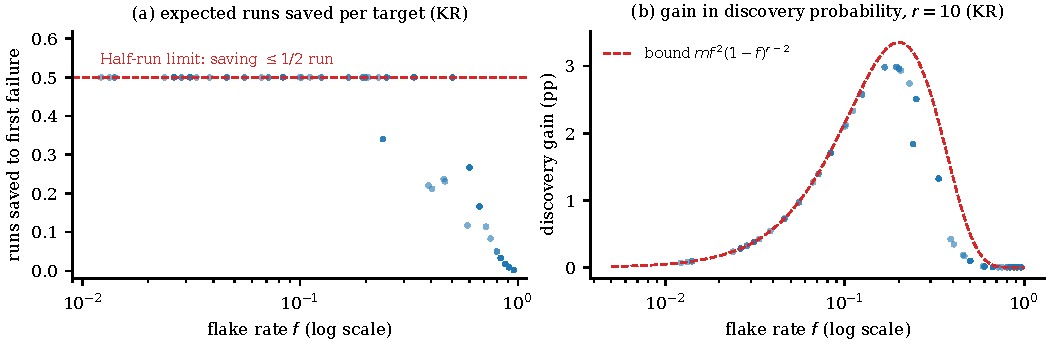
\includegraphics[width=\textwidth]{figures/pertest_S1.pdf}
\caption{Per-test benefit of independent reversal pairs versus flake rate (KR, S1). (a) Expected runs saved until the first failure: \NBzero{} tests sit exactly on the half-run limit of Theorem~\ref{thm:half}. (b) Gain in detection probability after 10 runs against the rare-failure bound in Section~\ref{sec:theory}; most tests lie on the bound because $B\approx0$.}
\label{fig:pertest}
\end{figure*}

\textbf{But it saves less than half a run.} \NBzero{} tests have $B=0$ and save exactly half a run (Fig.~\ref{fig:pertest}(a)). On average pairing saves \KRSaveMean{} runs: \KRRunsIID{} under \IIDp{} versus \KRRunsPair{} under \PAIRp{} (NR: \NRSaveMean{} runs). At fixed budgets the average per-test gain is \KRGainTwo\pp{} at $r=2$, but only \KRGainTen\pp{} at $r=10$ and \KRGainTwenty\pp{} at $r=20$ (KR). The gain follows the rare-failure bound of Section~\ref{sec:theory} closely (Fig.~\ref{fig:pertest}(b)): it peaks near $f=1/r$ and vanishes for frequently failing tests, which are found anyway. Reversal thus already delivers nearly all that independent pairs can deliver.

\begin{table}[t]
\caption{The limits map on real data: expected runs to the first failure (KR), averaged over all \NTargets{} OD tests and over the \NflowTen{} rare ones ($f<0.1$).}\label{tab:map}
\centering\small
\setlength{\tabcolsep}{3pt}
\begin{tabular}{@{}lrr@{}}
\toprule
Schedule (theorem) & all & rare\\
\midrule
\IIDp{} ($1/f$) & \ETIid & \ETIidRare\\
\PAIRp{}, outcome-blind (Thm.~\ref{thm:block}, exact) & \ETPair & \ETPairRare\\
4-run blocks (lower bound) & \ETBlockfour & \ETBlockfourRare\\
reverse-or-fresh (per-target oracle) & \ETOracle & \ETOracleRare\\
uniform marginals (lower bound) & \ETUniform & \ETUniformRare\\
\bottomrule
\end{tabular}
\end{table}

\textbf{The misses, and the headroom, are rare tests.} At $r=10$ and $r=20$, \KRShareLowTen\% and \KRShareLowTwenty\% of the \IIDp{} misses come from the \NflowTen{} tests with $f<0.1$. Most are brittles and single-polluter victims: they have $B=0$, but fail rarely. Table~\ref{tab:map} places the averages on the map of Section~\ref{sec:theory}. The uniform-marginal bound lies \HeadroomUniformPct\% below \IIDp{}, and pairing closes \HeadroomShare\% of that gap. For the rare tests, \IIDp{} needs \ETIidRare{} runs and the bound is \ETUniformRare. Per-target optima may conflict, so the gap bounds what any detector could save rather than offering a saving. Closing a fixed fraction $\eta$ of it with independent blocks requires $k\ge1+2\eta/f$ runs per block.

\textit{Answer:} Pairing is safe for all \NTargets{} models, and saves \KRSaveMean{} runs per test on average, below 1\pp{} of detection from 10 runs on. The remaining headroom lies with rare tests and needs longer-horizon or information-directed designs.

\begin{table}[t]
\caption{Suite-level detection (\% of \NTargets{} OD tests) and differences in percentage points with 95\% CI half-widths (S1).}\label{tab:suite}
\centering\small
\setlength{\tabcolsep}{2.4pt}
\resizebox{\columnwidth}{!}{%
\begin{tabular}{@{}lrrrrr@{}}
\toprule
Budget $r$ (runs) & 2 & 4 & 10 & 20 & 40\\
\midrule
\csname @@input\endcsname generated/table_suite_S1.tex 
\end{tabular}}
\end{table}

\subsection{RQ2: The Deployed Gate}
Table~\ref{tab:suite} compares the four policies on complete modules.

\emph{Differences are confined to tiny budgets.} Under KR, \PAIRp{} improves on \IIDp{} by \KRPairMinusIidTwo\pp{} at $r=2$ and \KRPairMinusIidFour\pp{} at $r=4$, but only by \KRPairMinusIidTen\pp{} at $r=10$ and \KRPairMinusIidTwenty\pp{} at $r=20$ (NR: \NRPairMinusIidTwo, \NRPairMinusIidFour, \NRPairMinusIidTen, \NRPairMinusIidTwenty\pp).

\emph{The gate is never significantly worse than random orders.} This holds in every module, under both protocols, at every budget from 1 to 40 runs; the most negative module-level $z$-score is $-1.0$ before any multiple-comparison correction. From 10 runs on, \GATEp{} and \PAIRp{} differ by at most 0.11\pp{} in aggregate, with signs that vary by module. Under NR the gate almost always reverses after the first round, because one run cannot reveal both outcomes.

\emph{The gate costs detection only with a tiny budget and a passing reference.} There the first round often finds something new, so \GATEp{} skips the reversal and trails \PAIRp{} by \KRPairMinusGateTwo\pp{} at $r=2$. \STRICTp{} is weaker still, because a run without any failure is rare in modules with many OD tests. Per module (supplement), reversal adds at most about 1\pp{} at $r=10$ under KR. The largest effects ($+3.0$\pp, NR) occur where OD tests fail in most orders, so that detection waits for a \emph{passing} run.

\textbf{The real tool.} We also ran the unmodified iDFlakies (commit f54b3f0) on the two frequently failing executed modules of RQ3, together with two minimal patches of its decision code: one never reverses (\IIDp), and one reverses after every fresh order (\PAIRp). Every variant made 20-round detector runs with shared seeds (\IdfRunsAis{} per variant on \texttt{aismessages}, \IdfRunsHttp{} on \texttt{http-request}; \IdfDetectorRuns{} runs in total), under a protocol frozen before the first run. The simulation matches the tool. All \IdfOrders{} executed orders were class-contiguous permutations of the module. The gate reversed exactly when our rule predicts, in all \IdfGateTransitions{} decisions. All \IdfComparisons{} target outcomes on the tool's own orders matched S1. Table~\ref{tab:idflakies} gives the measured contrasts. On \texttt{aismessages} they reproduce the simulation (e.g., \GATEp$-$\IIDp{} at $r=2$: $+6.1$\pp{} measured, $+5.7$\pp{} simulated). On \texttt{http-request}, the tool's own reference order fails 15 of the 25 targets in its runner, although native Maven passes them. Round-0 \emph{passes} of those targets then count as new detections, so the gate never reverses in round~1 and forgoes most of reversal's benefit at small budgets. This is the suite-level dependence of Section~\ref{sec:theory}-C, observed in the deployed tool.

\begin{table}[t]
\caption{Real iDFlakies runs: detection difference in percentage points of the module's targets (KR, mean and 95\% bootstrap CI over paired detector runs).}\label{tab:idflakies}
\centering\small
\setlength{\tabcolsep}{2.5pt}
\resizebox{\columnwidth}{!}{%
\begin{tabular}{@{}llccc@{}}
\toprule
Module & Contrast & $r=2$ & $r=4$ & $r=10$\\
\midrule
\csname @@input\endcsname generated/table_idflakies.tex
\bottomrule
\end{tabular}}
\end{table}

\textbf{Robustness.} Under S2 the suite contrasts change by at most 0.04\pp{} at any budget. Scoring only the \NConsistent{} reference-consistent targets gives \PAIRp{}$-$\IIDp{} at $r=10$ of \KRConsPairMinusIidTen\pp{} (KR) and \NRConsPairMinusIidTen\pp{} (NR). Weighting modules equally gives \KRMWPairMinusIidTen\pp{} and \NRMWPairMinusIidTen\pp. The supplement has the tables.

\textit{Answer:} From 10 runs on, all reversal policies are within 1\pp{} of random orders, and the deployed gate is never significantly worse; the real tool confirms both the simulated gate rule and these magnitudes. At budgets of two to four runs, unconditional pairing is better, especially when the tool's reference order does not pass.

\subsection{RQ3: Real Executions}\label{sec:execution}
RQ1 and RQ2 rest on the published polluter/cleaner models. We therefore executed complete modules and compared each real outcome with the model's prediction for the same order.

\textbf{Protocol.} Before building anything, we froze the modules, fallbacks, seeds, sample sizes, and stopping rules. Selection could not depend on model agreement. The primaries were \texttt{aismessages} (two targets, model $f=2/3$, $B=1/3$) and \texttt{http-request/lib} (25 targets, six reference-inconsistent, $f=1/3$, $B=0$). Both built at the dataset revisions without changes to code, tests, dependencies, or fixtures, and their native test inventories matched the recorded ones exactly (44 and 163 tests). Every execution ran the complete module in a fresh JVM with normal class and method fixtures. An ordered JUnit runner kept whole-class execution and checked each actual test start against the requested order. The formal sample has 300 independent uniform class-contiguous orders per module, each followed by its reversal. All \ExecRuns{} formal executions were valid, with exact order agreement and no skips or timeouts. \ExecPilotRuns{} pilot runs (three repetitions of the recorded order, and five random orders twice each) were stable and are excluded.

\textbf{Rare failures.} Both modules have $f\ge1/3$, whereas our argument concerns rare failures. A second protocol, frozen before any build, therefore added \texttt{marine-api} (\ExecRareTests{} tests, \ExecRareTargets{} targets, model $f=1/32$, $B=0$) with \ExecRarePairs{} pairs and a fixed fallback order. It built unchanged, and no fallback was needed. Before the formal sample, the runner gained method-order control for one JUnit~3 class, and it now accepts the one natively ignored test; the package documents both. All \ExecRareRuns{} formal executions were valid.

\begin{table}[t]
\caption{Real executions: complete-suite size / OD targets, independent pairs, ranges of observed anchor $f$ and joint $B$ across targets, and S1 mismatches / target outcomes. These ranges are not confidence intervals.}\label{tab:execution}
\centering\small
\setlength{\tabcolsep}{2.5pt}
\resizebox{\columnwidth}{!}{%
\begin{tabular}{@{}lrrrrr@{}}
\toprule
Module & tests/OD & pairs & $\hat f$ & $\hat B$ & mismatch\\
\midrule
\csname @@input\endcsname generated/table_execution.tex
\csname @@input\endcsname generated/table_execution_rare.tex
\bottomrule
\end{tabular}}
\end{table}

\textbf{Every outcome matches.} All \ExecAllComparisons{} target outcomes matched S1 and S2 order by order (Table~\ref{tab:execution}), which is stronger than matching failure rates. In \texttt{marine-api}, targets failed in only \ExecRareFailingDirections{} of \ExecRareDirections{} executions, and the model predicted each of these failures and every pass. With the pair as the independent unit, zero mismatching pairs bound the mismatch probability (one-sided 95\%) by $1-0.05^{1/300}\approx0.0099$ in the first two modules and by \ExecRareZeroBound{} in \texttt{marine-api}. There the model's $f=1/32$ lies inside every target's 95\% interval (observed \ExecRareFMin--\ExecRareFMax), and no pair failed in both directions. The 12 targets fail in correlated groups, so they are not 12 independent confirmations. For \ExecMarginalOutside{} of the 27 targets in the first two modules, the model's theoretical $f$ lies outside the observed 95\% interval, but the model has the identical rate on the same sampled orders; this is sampling variation, not disagreement.

\textbf{The recorded original order really fails.} Native Maven runs passed every test, but executing the recorded original order failed the six reference-inconsistent \texttt{http-request} targets in all three repetitions, exactly as S1 and S2 predict. For these targets the model is right and the historical passing reference does not reproduce.

\textbf{The dataset misses OD tests.} Three \texttt{http-request} tests outside the published targets also failed in about a third of the orders. They behave exactly like the module's 25 known victims. The same polluter and cleaner, which set and reset a static connection factory, explain all 613 recorded runs and 14 targeted confirmation runs. We report them but keep them out of the target set.

\textit{Answer:} The abstraction predicts every sampled outcome of the \ExecAllTargets{} executed targets exactly, in the rare regime as well as for frequently failing and reference-inconsistent targets. It also explains three OD victims that the dataset missed.

\section{Discussion}\label{sec:discussion}
\textbf{For tool builders: keep the gate, and stop tuning reversal.} At iDFlakies' default budgets, the gate, unconditional pairing, and random orders differ by less than 1\pp, and the gate is never significantly worse than random. Only when a per-commit budget is two to four runs does unconditional pairing pay off: by \KRPairMinusGateTwo\pp{} over the gate at $r=2$ in simulation, and by up to 12.5\pp{} in the real tool when its reference order does not pass. Beyond that, no reversal variant can help much. Independent pairs save at most half a run per test, and blocks of $k$ runs at most $(k-1)/2$. These limits need only uniform marginals, not our OD model, so they hold whatever the tests do.

\textbf{For rare OD tests: buy information, or coordinate longer horizons.} Rare tests cause almost all misses, and the dataset's OD tests were themselves found by earlier detectors, so rare ones are probably underrepresented. Equation~\eqref{eq:predictor} tells a reversal predictor what it must achieve: $sJ(1-f)>f(c+aq)$. Shared-state analysis~\cite{gyori2015poldet,bell2015electrictest,gambi2018pradet} and prioritisation~\cite{iqbal2025ftw} are candidate sources of that information. Covering designs over about $1/f$ runs~\cite{wei2021tacas,li2023issta} are the other way past the block limit.

\textbf{For evaluators: separate model, simulator, and execution.} Agreement with a reference simulator checks only the simulator; real executions check the model. Evaluate outcome-gated policies jointly over a module, because no per-target statistic determines them (Proposition~\ref{prop:gate}), and state the passing-reference assumption.

\section{Threats to Validity}\label{sec:threats}
\textbf{Construct.} The 47-module results rest on the polluter/cleaner abstraction of prior work~\cite{wei2021tacas,li2023issta}. RQ3 checks it against real executions, but only for the sampled orders of the executed modules. The dataset lists no polluter groups, so OD tests that need several polluters jointly are not represented. We ignore non-OD flakiness, failures that alter later behaviour, confirmation reruns, the tool's reuse of historical orders, and wall-clock cost.

\textbf{Population.} The dataset's OD tests were found by earlier detectors, so rarely failing OD tests are probably underrepresented, and RQ3 found three victims it misses. Both effects make our finding that rare tests dominate the misses conservative.

\textbf{Theory.} Theorem~\ref{thm:cov} covers every S1 model in the dataset; this is a statement about the recorded models. The general class-contiguous case remains a conjecture, checked exhaustively up to seven tests. The proofs are complete, and the package checks their consequences exhaustively on small instances (14{,}791 hierarchy models, 731{,}630 orders) and verifies the budget and hitting-time identities in exact arithmetic.

\textbf{External.} The simulation covers 47 Maven modules and one tool at one commit. Execution covers feasibility-selected modules in one Linux/JDK environment. Other frameworks also nest tests (e.g., describe blocks in Jest~\cite{hashemi2025js}), and Theorem~\ref{thm:cov}(a) covers arbitrary nesting, but the empirical magnitudes may differ.

\section{Related Work}\label{sec:related}
\textbf{OD test detection.} DTDetector introduced reversal, randomised, and bounded exhaustive detection~\cite{zhang2014dtdetector}. iDFlakies randomises class-contiguous orders and classifies flaky tests~\cite{lam2019idflakies}. Other work detects state pollution or test dependencies directly~\cite{gyori2015poldet,bell2015electrictest,gambi2018pradet}, repairs OD tests~\cite{shi2019ifixflakies}, or detects them incrementally~\cite{li2022incidflakies}. Empirical studies cover Python~\cite{gruber2021python} and JavaScript~\cite{hashemi2025js}; see Parry et al.~\cite{parry2021survey} for a survey. Systematic approaches cover test pairs with Tuscan squares~\cite{wei2021tacas,li2023issta}. Li et al.\ found that most generated orders are unnecessary and called for prioritisation~\cite{li2023issta}, which Iqbal et al.\ pursue~\cite{iqbal2025ftw}.

\textbf{Probabilistic analysis of test orders.} Wei et al.\ derived flake rates for special cases and proposed the reversal change~\cite{wei2021tacas}. Wang et al.\ count failing orders with Alloy~\cite{wang2021alloy}. We prove the reversal inequality in general hierarchies, bound its value, and separate per-test from suite-level claims.

\textbf{Antithetic sampling.} Pairing a sample with a reflected one is the classical antithetic technique~\cite{hammersley1956antithetic,owen2013mc}, and its use for estimating probabilities is well studied~\cite{snijders1984antithetic}. Those results reduce estimator variance, and they help only when the pair is negatively correlated. Theorem~\ref{thm:cov} establishes that sign for OD-test semantics, using a certificate for hierarchies and Harris' correlation inequality~\cite{harris1960} for unconstrained orders. The sign is not generic (Table~\ref{tab:classify}). Theorem~\ref{thm:half} and Eq.~\eqref{thm:both} concern detection times rather than estimator variance.

\section{Conclusion}\label{sec:conclusion}
Reversal's value is bounded, even when its intuition is correct: independent pairs save at most half a run per target's first failure, and independent small blocks cannot deliver constant-factor savings for rare failures. Under explicit OD-model hypotheses, pairing is safe; a suite-level gate is a different policy and does not inherit that guarantee. Simulation of \NTargets{} published models finds gains below 1\pp{} from 10 runs on. Real executions of three modules match all \ExecAllComparisons{} predicted outcomes of \ExecAllTargets{} targets, including rarely failing ones. Our predictor tradeoff makes the next question concrete: can useful failure information be obtained accurately and cheaply enough to outperform outcome-blind sampling?

\section*{Acknowledgment}
We thank GPT and Codex (OpenAI) and Claude (Anthropic), which helped us push the theory forward. They carried out much of the mathematical derivation for cases (b)--(d) of the safety theorem, wrote most of the simulation, verification, and execution code, and helped draft and polish the text. Gemini (Google) helped with the literature search. We then checked every proof and the idea behind it ourselves, cross-checked the derivations with independent exact computations, verified every citation against its source, and regenerated all numbers from the released scripts. We take full responsibility for the content.

\section*{Data Availability}\label{sec:data}
The anonymized replication package is available at \url{https://anonymous.4open.science/r/tset-71C0}. It contains the complete proofs, exact verification scripts, the suite simulator, the analysis scripts that generate every number, table, and figure in this paper, the real-execution protocol, runner, and measurements, and the processed dataset of Li et al.~\cite{li2023issta} with provenance.

\bibliographystyle{IEEEtran}
\bibliography{references}

\end{document}
